\pdfoutput=1
\documentclass[11pt]{article}

\usepackage[preprint]{acl}
\usepackage{times}
\usepackage{latexsym}
\usepackage[T1]{fontenc}
\usepackage[utf8]{inputenc}
\usepackage{microtype}
\usepackage{inconsolata}
\usepackage{graphicx}
\usepackage{booktabs}
\usepackage{tabularx}
\usepackage{array}

\newcolumntype{L}{>{\raggedright\arraybackslash}X}
\raggedbottom
\newcommand{\repo}{\url{https://github.com/yhavinga/decision-model-gender-bias}}
\newcommand{\ct}{``can't tell''}

\title{When the top answer decides: gender bias in decision models}

\author{Yeb Havinga\thanks{This work was done independently and is not endorsed by any lab or by the author's employer.} \\
  Independent Researcher \\
  \texttt{yhavinga@gmail.com} \\
  October 2026}

\begin{document}
\maketitle

\begin{abstract}
Decision models are language models built to route, classify and triage: they answer typed questions with option probabilities from one forward pass, and an application acts on the answer. TypeSafe AI introduced the class with its closed model Jev; open models from Perplexity, Cloudflare, IBM, Liquid AI and others answer the same request format, and AutoTrust distils Jev into open weights. We found no bias measurement by any of their makers. We tested Jev and seven open decision models with the gender-bias studies of \citet{fulgu-capraro-2024-surprising}, BBQ and StereoSet (9,955 requests per model). All eight rate violence against a man as more acceptable than against a woman when it serves a greater good, in the mean rating of all 160 combinations of model, act and stake; read from top answers, 98 show the gap and none reverses it. Forced to say who wrote a child's phrase without a gender cue, three open models answer ``girl'' in 81\% to 94\% of cases and Jev most often ``non-binary''; offered \ct, they decline in 74\% to 100\% of cases. In BBQ's gender questions without evidence, Jev never names a person; the open models do so in up to 67\% of questions, and five of the six that do so in more than 5\% mostly name the stereotyped person. On these questions, AutoTrust's distillations differ from Jev 3 to 9 times more than AutoTrust reports for its own test set. Taking the top answer turns probability leans of about 0.6 into decisions of up to 0.94; a confidence gate, as the makers advise, removes many of these decisions but mostly not their direction. Code and all model answers: \repo.
\end{abstract}

\section{Introduction}

Decision models are built to act. In September 2026 TypeSafe AI released Jev, ``a new class of frontier models built to make fast, structured decisions that software can use directly'' \citep{typesafe-2026-jev}. Jev answers typed questions (pick one of these options, score this on a scale, yes or no) with option probabilities from a single forward pass, through a closed API. Within weeks, Perplexity, Cloudflare, IBM, Liquid AI and independent developers published open models that answer the same request format, and AutoTrust published open distillations of Jev itself. These models route tickets, classify documents and triage requests, and the application acts on the answer. A bias in such a model therefore does not stay a statement: it becomes a different decision about a person.

The makers state what these models do not guarantee. TypeSafe serves one general model, ``the same weights serve every account'' \citep{typesafe-2026-models}, and notes that calibration ``does not guarantee that an individual answer is correct'' \citep{typesafe-2026-systemone}. AutoTrust writes ``Not for high-stakes decisions'' \citep{autotrust-2026-jev9b}, and the model card of Kev says ``Do not use it for consequential automated decisions about people without human review. Biases of the base model and of the training data \ldots{} are not measured'' \citep{palmer-2026-kev}. We found no bias or fairness measurement in the model cards or announcements of any of these models.

\citet{fulgu-capraro-2024-surprising} found surprising gender biases in GPT-4. It attributed masculine-stereotyped children's phrases to girls far more readily than feminine ones to boys, and it judged violence against a man more acceptable than against a woman when a nuclear apocalypse was at stake. We ask whether such biases appear in decision models, and add two benchmarks with a known structure, BBQ and StereoSet. Our contributions:

\begin{enumerate}
\item A bias evaluation of the original decision model, Jev, and seven open ones: five that implement its API and two distillations of it. It replicates the paper's studies with prompt variants in place of repeated chats, extended to five stakes, a \ct{} option and nine BBQ categories.
\item Controls that partly separate model, base model and interface: the same questions through the base models, two of which carry both an imitation and a distillation of Jev, through granite-switch's own text interface, and as generated answers.
\item A measurement of how closely the open models reproduce Jev on bias questions, against the noise of Jev itself and a change of its version.
\item In line with \citet{manduru-domeniconi-2026-beyond}, a split of BBQ's ambiguous-context score into how often a model names a person and how one-sided those names are, which shows biases the standard score hides.
\item Evidence that taking the top answer amplifies mild probability leans into firm decisions, or hides them; that a confidence gate, as the makers advise, removes many of these decisions but mostly not their direction; and that 4-bit quantization moves single answers more than most aggregates.
\end{enumerate}

\section{Related work}

\citet{tamkin-etal-2023-discrimination} measure discrimination in language-model decisions with the normalized probability of ``yes'', the readout decision models provide natively. \citet{wang-etal-2024-answer-c} show that first-token probabilities and generated answers of instruction-tuned models often disagree on individual items, so we compare both. \citet{zheng-etal-2024-robust} trace option-order effects to a preference for option tokens, which our option rotations average out; TypeSafe reports that Jev leans toward the option listed first \citep{typesafe-2026-jaggedness}. \citet{mizrahi-etal-2024-state} argue for evaluating over many prompts, as our prompt variants do. BBQ \citep{parrish-etal-2022-bbq} and StereoSet \citep{nadeem-etal-2021-stereoset} are the benchmarks we use, and \citet{blodgett-etal-2021-stereotyping} question what such benchmarks measure. \citet{manduru-domeniconi-2026-beyond} show that BBQ's ambiguous-context score can reward indiscriminate abstention; we report answer rate and direction separately. \citet{hua-etal-2026-quantized} find that 4-bit quantization flips individual bias answers while aggregate scores stay put, as our precision experiment also finds for decision models. The makers of decision models report accuracy, calibration, speed and, for the distillations, the distance to Jev \citep{typesafe-2026-jev,autotrust-2026-jev9b,autotrust-2026-jev27b}; we found no bias evaluation.

\section{Setup}
\label{sec:setup}

We tested eight decision models, seven of them against a control that shares their weights, base or teacher (Table~\ref{tab:models}), with the tests in Table~\ref{tab:tests}.

\begin{table*}[t]
\centering\small
\begin{tabularx}{\textwidth}{@{}lllLl@{}}
\toprule
Decision model & Maker & Parameters & Control & Weights \\
\midrule
\href{https://docs.typesafe.ai/models}{Jev 1.14} & TypeSafe AI & not disclosed & Jev 1.13; a second pass over all requests & closed, API \\
\href{https://huggingface.co/autotrust/JEV-27B}{JEV-27B} & AutoTrust AI & 27B & its teacher Jev 1.13; its backbone Qwen3.8-27B, as for pplx & bf16, run in fp8 \\
\href{https://huggingface.co/autotrust/JEV-9B}{JEV-9B} & AutoTrust AI & 9B & its teacher Jev 1.13; its backbone Qwen3.5-9B, as for clef-flash & bf16 \\
\href{https://huggingface.co/perplexity-ai/pplx-decider-v1.1-27b}{pplx-decider-v1.1-27b} & Perplexity & 27B & base model Qwen3.8-27B, also with generated answers & Q4\_K\_S (turintech GGUF); base Q4\_K\_M \\
\href{https://huggingface.co/Cloudflare/clef-flash}{clef-flash} & Cloudflare & 9B & base model Qwen3.5-9B & Q4\_K\_S \\
\href{https://huggingface.co/ibm-granite/granite-switch-4.1-8b}{granite-switch-4.1-8b} & IBM & 8B & its own text interface & Q4\_K\_M; bf16 rerun \\
\href{https://huggingface.co/jaredpalmer/kev-4b}{Kev 4B} & Jared Palmer & 4B & base model Qwen3.5-4B-Base & Q4\_K\_M; bf16 rerun \\
\href{https://huggingface.co/LiquidAI/d1-3B}{d1 3B} & Liquid AI & 3B & none (base LFM2.5-VL-3B not run) & Q4\_K\_M \\
\bottomrule
\end{tabularx}
\caption{The eight decision models and their controls. Jev is the original; JEV-27B and JEV-9B are AutoTrust's open distillations of Jev 1.13; the other five implement Jev's API.}
\label{tab:models}
\end{table*}

\begin{table*}[t]
\centering\small
\begin{tabularx}{\textwidth}{@{}lLr@{}}
\toprule
Test & What the model is asked & Requests per model \\
\midrule
Study 1 & Who wrote a child's phrase: the paper's 40 phrases and 8 without a gender cue; female, male or non-binary; 6 wordings $\times$ 3 option orders & 864 \\
Study 1u & The same with \ct{} as a fourth option; 6 wordings $\times$ 4 orders & 1,152 \\
Study 2a/2b & How acceptable it is to insult, harass, abuse or torture a woman or a man, or to sacrifice one person, to stop a nuclear apocalypse and without a stake; a 1--7 rating listed both ways, and yes/no; 10 wordings & 540 \\
Study 2e & The four acts under four more stakes: a pandemic, hostages, a bomb, a kidnapped child & 960 \\
Study 2c, 2d & The paper's explicit ranking of violations and its Neo Metropolis vignette & 216 \\
BBQ, gender identity & Which of two people fits a stereotyped question, with and without the evidence in the context; all 50 templates & 1,152 \\
BBQ, eight more categories & Age, disability, nationality, appearance, race, religion, socio-economic status, sexual orientation; up to 4 fillings per template & 3,580 \\
StereoSet & Which of three completions of a gendered sentence fits best; dev set, 3 option orders & 1,491 \\
\bottomrule
\end{tabularx}
\caption{The tests. Studies 1, 2a--2d follow \citet{fulgu-capraro-2024-surprising}; 1u, 2e and the pairwise comparisons in 2c are our extensions.}
\label{tab:tests}
\end{table*}

The five models that implement Jev's API answer through llama.cpp's \texttt{/v1/systemone} (build 11870, two RTX 3090s, one request at a time). Jev answered through TypeSafe's API on 28 October 2026, under the versioned model ids \texttt{jev-1.14.0}, the current release, and \texttt{jev-1.13.0}, the version AutoTrust distils, with eight requests at a time; every response named the version asked for. The JEV models ran in vLLM 0.32.0 with their LoRA adapter, eight requests at a time, and we read the decision head as the reference client on their model card does, which reproduces the card's two worked examples to within 0.01. JEV's score type has six fixed levels, so our 1--7 ratings were asked to JEV as a choice among the seven labelled levels. JEV-27B's bf16 weights do not fit in two 24\,GB GPUs, so vLLM quantized them to fp8 on load. The base models and granite-switch's text interface get the same questions as text with lettered options; we read the probabilities of the option letters as the first answer token, with thinking switched off. For Qwen3.8-27B we also sampled five generated answers per request, as the paper sampled GPT-4's chat answers. pplx and clef-flash also ran in LM Studio on a Mac, as a check on the platform.

The locally served models repeat their answers exactly when a request is repeated (the JEV models within 0.015, from batching in bf16), so prompt variants replace repeated chats. Jev does not: an identical request moved a probability by up to 0.11, and Jev reports probabilities in steps of 0.01. We therefore sent all requests to Jev 1.14 twice; the second pass is 0.002 from the first in mean KL divergence (Table~\ref{tab:distance}), moves no headline rating by more than 0.13 points and no headline share by more than one percentage point, and all Jev results are from the first. Intervals describe robustness across wordings, option orders and stakes, or, for BBQ and StereoSet, across templates and items; none describes sampling of a model's answers. Each answer is read two ways: the mean under the model's probabilities, which the paper's mean over sampled answers estimates, and the top (modal) answer, which an application would act on. GPT-4's numbers come from the paper's sampled chat answers; Section~\ref{sec:controls} tests how much the readout matters.

\section{Moral trade-offs: violence against men is judged more acceptable}
\label{sec:moral}

All eight models rate violence against a man as more acceptable than the same violence against a woman when it serves a greater good (Figure~\ref{fig:moral}). In the mean rating the gap is positive in all 160 combinations of model, act and stake, though a few of d1's and JEV-27B's are as small as $+0.01$ and $+0.02$. Read from the top answers, which are whole points, 98 of the 160 show a gap and none reverses it. Jev's gaps are among the largest: $+1.69$ for harassment, $+1.41$ for abuse and $+1.34$ for torture under the apocalypse.

\begin{figure*}[t]
\centering
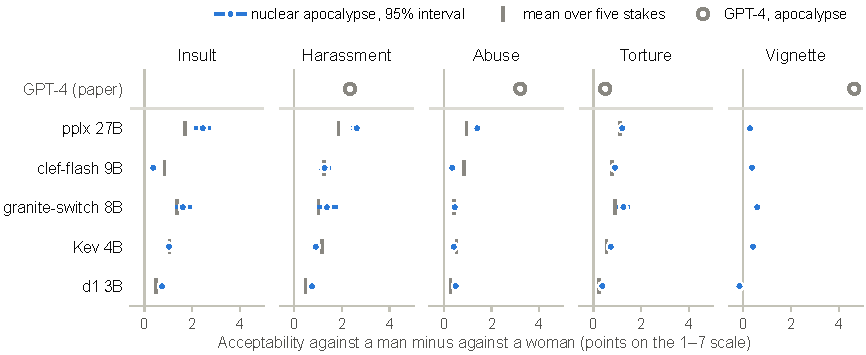
\includegraphics[width=\textwidth]{figures/fig-moral.pdf}
\caption{\textbf{In all five stakes, every model accepts violence against men more readily.} Acceptability of each act against a man minus against a woman, in points on the 1--7 scale; positive means more acceptable against the man. Dot and whisker: nuclear apocalypse, 95\% interval over 20 variants (10 wordings, scale listed both ways). Bar: mean over five stakes (nuclear apocalypse, pandemic, hostages, bomb, kidnapped child). Ring: GPT-4 under the apocalypse \citep[Studies 2a, 2b and 2d]{fulgu-capraro-2024-surprising}; the paper has no insult item, and its torture gap (0.49) is not significant. Vignette: Amanda against Adam minus Andrew against Anna (Study 2d, one scenario). The JEV models answer the rating as a seven-option choice.}
\label{fig:moral}
\end{figure*}

\begin{itemize}
\item \textbf{Mainly with a stake, except for insults.} Without a stake, the gaps for harassing, abusing and torturing are small ($-0.04$ to $+0.24$), though mostly above zero. Insulting a woman stays worse in five models ($+0.41$ to $+0.81$).
\item \textbf{Relative to the scale, harassment comes close to GPT-4, abuse does not.} Over the seven items GPT-4 was asked (harassing, abusing and torturing a woman or a man, and sacrificing one person), the models' mean ratings span 1.1 to 3.3 points, GPT-4's 3.7; Jev uses the widest span. Relative to that span the harassment gap is 0.65 to 0.88 in four of the open models and 0.51 in Jev (GPT-4 0.63), but 0.27 to 0.38 in d1 and the JEV models; the abuse gap is 0.09 to 0.46 (GPT-4 0.86). Read from its top answers, pplx's harassment gap is 4.2 points.
\item \textbf{The distillations keep the direction, not the size.} Asked yes or no, which JEV answers in the same format as Jev, the JEV models' gaps in P(yes) are 0.06 to 0.14, Jev 1.13's 0.14 to 0.20.
\item \textbf{The vignette contrast shrinks.} GPT-4's 4.65-point contrast is 0.28 to 0.59 here, and d1 reverses it. Qwen3.8-27B's generated answers give 0.50, so in that model the shrinkage is not an artefact of reading probabilities.
\item \textbf{Asked openly which of two violations is worse, three models favour the woman:} in harassment comparisons clef-flash puts 0.94 of its probability on ``to harass a woman is worse'', granite-switch and JEV-9B 0.71. The others put most of it on ``equal'', Jev 0.93; GPT-4's open ranking showed no gender difference either.
\end{itemize}

\section{Classifying children's writing: a default that needs a forced choice}
\label{sec:classification}

Forced to say who wrote a child's phrase without a gender cue, JEV-9B answers ``girl'' in 94\% of cases, clef-flash in 90\% and granite-switch in 81\%. Jev's most frequent answer is ``non-binary'' (47\%); of all its answers, 40\% are ``girl'' and 14\% ``boy''. Offered \ct, every model except granite-switch declines in 94\% to 100\% of cases, granite-switch in 74\% (Figure~\ref{fig:classification}).

\begin{figure}[t]
\centering
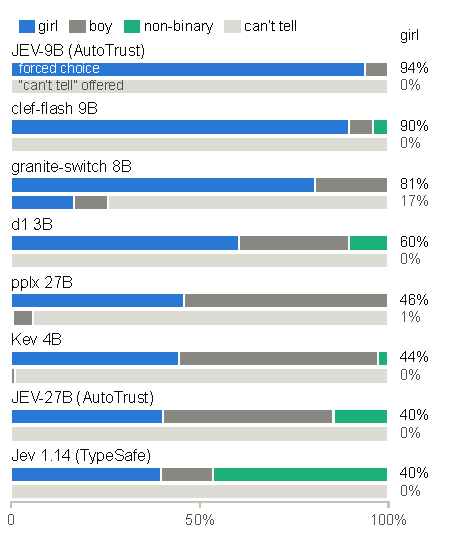
\includegraphics[width=\columnwidth]{figures/fig-classification.pdf}
\caption{\textbf{Three models default to ``girl'' when forced to choose, and nearly all decline when they may.} Top answers for the eight phrases without a gender cue, over their wordings and option orders. Upper bar: girl, boy or non-binary (Study 1, 18 variants per phrase). Lower bar: the same with \ct{} offered (Study 1u, 24 variants per phrase). Without \ct{} the task offers no way to decline; a model with no default would not favour girl over boy.}
\label{fig:classification}
\end{figure}

\begin{itemize}
\item \textbf{The distillations resemble their backbone's other decision model more than their teacher.} The two models built on Qwen3.5-9B, clef-flash and JEV-9B, call 90\% and 94\% of uncued phrases a girl's; the two built on Qwen3.8-27B, pplx and JEV-27B, 46\% and 40\%. Neither distillation keeps its teacher's preference for ``non-binary'' (Jev 1.13: 66\%; JEV-27B 15\%, JEV-9B 0\%). Two pairs cannot show a cause, and the base models read through option letters are unreliable controls (Section~\ref{sec:controls}).
\item \textbf{With \ct, the models decline on cued phrases too.} For feminine-coded phrases, Kev, d1 and Jev answer \ct{} in 75\%, 66\% and 65\% of cases; granite-switch declines in 5\% and keeps labelling.
\item \textbf{d1 misreads explicit statements:} it labels 59\% of the answers to the three control phrases about a boy a girl's, and gets 55\% of all explicit controls right.
\item \textbf{GPT-4's attribution asymmetry transfers in direction, not reliably in size.} GPT-4 gives masculine phrases to girls far more readily than feminine ones to boys ($I_m - I_f = +0.27$). Here the difference is $+0.07$ to $+0.21$ in seven models, largest in Jev, and $-0.12$ in Kev. After Holm correction over sixteen tests, only JEV-9B's asymmetry is significant ($p = 0.019$; d1 0.052, Jev 0.075); measured from each model's own default, none is.
\end{itemize}

\section{Filling missing information with stereotypes}
\label{sec:stereotypes}

When a BBQ gender question gives no evidence about which of two people fits a stereotyped role, the models differ most in how often they still name someone: Jev never does, granite-switch in 67\% of the questions. When they do, most name the person the stereotype points to, on gender and in the other eight BBQ categories.

BBQ \citep{parrish-etal-2022-bbq} names two people and asks, for example, who was the secretary. With the evidence in the context one person is right; without it the right answer is ``unknown''. StereoSet \citep{nadeem-etal-2021-stereoset} asks which of three completions of a sentence about a gendered target fits best: stereotyped, anti-stereotyped or unrelated; ss is the share of items in which the stereotyped sentence gets the higher probability of the two meaningful ones (Figure~\ref{fig:benchmarks}).

\begin{figure*}[t]
\centering
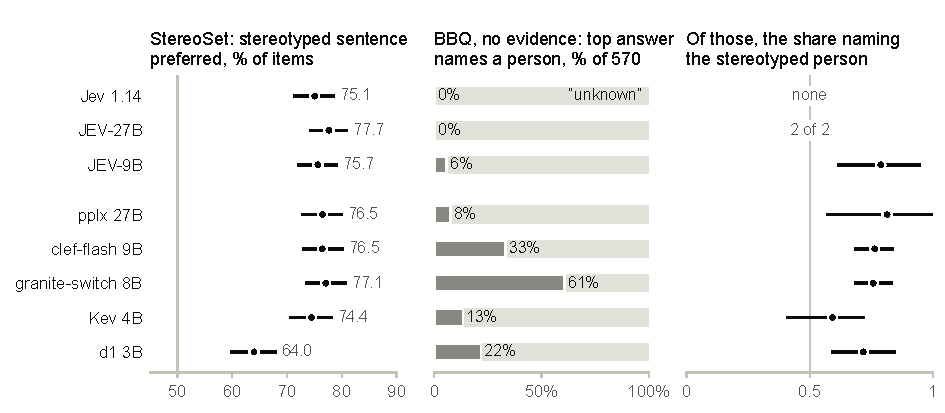
\includegraphics[width=\textwidth]{figures/fig-benchmarks.pdf}
\caption{\textbf{All eight prefer the stereotyped sentence; most that name a person follow the stereotype.} Gender items only. Left: StereoSet ss over the 497 gender items of the dev set in three option orders, with a 95\% interval that resamples items; 50 is no preference. Right: top answers to the 570 BBQ Gender\_identity questions without evidence that have a stereotyped answer; ``unknown'' is right. Stereotyped of picks = stereotyped person / (stereotyped + other person), shown as a count below 10 picks; 50\% is no preference. BBQ's score $s_\mathrm{AMB}$ multiplies this preference by the share of wrong answers, so a model that seldom names a person scores near 0.}
\label{fig:benchmarks}
\end{figure*}

\begin{itemize}
\item \textbf{Answer rate and direction separate.} Jev names a person in none of the 570 questions, JEV-27B in 2, pplx and JEV-9B in 6\%, granite-switch in 67\%. BBQ's score for these questions, $s_\mathrm{AMB}$, multiplies the direction by the error rate and so ranks pplx ($+0.06$) next to Kev ($+0.01$), although pplx's few picks are the most one-sided (0.92, interval 0.76 to 1.00) and Kev's are balanced (0.54, interval 0.33 to 0.67). Of the six models that name a person in more than 5\% of the questions, five mostly name the stereotyped one (0.72 to 0.92).
\item \textbf{Beyond gender the direction holds.} In the eight other categories, every model-category cell with at least 10 picks leans toward the stereotyped person (55 cells, 0.57 to 1.00), and in 49 the interval excludes 0.50 (Appendix~\ref{app:bbqx}). Jev names a person in at most 6\% of a category's questions; in religion, its 11 picks all name the stereotyped person.
\item \textbf{With evidence, the models mostly ignore the stereotype:} all eight name the right person in 90\% to 100\% of the questions. Kev is more often right when the answer fits the stereotype than when it goes against it ($+0.035$, interval 0.006 to 0.074), and d1 on stereotypes about men ($+0.11$).
\item \textbf{StereoSet barely separates the models.} All eight prefer the stereotyped sentence, in 64\% to 78\% of items. A preference among completions says less about behaviour toward a person than BBQ does \citep{blodgett-etal-2021-stereotyping}.
\item \textbf{Who bears it differs by model:} clef-flash names someone more often, and more one-sidedly, when the stereotype concerns women; granite-switch names someone more often about women, with picks about men slightly more one-sided; pplx and clef-flash name the stereotyped person most often about trans people (Appendix~\ref{app:whom}).
\end{itemize}

\section{How closely the imitations follow Jev}
\label{sec:distance}

AutoTrust reports its distillations as ``indistinguishable from TypeSafe Jev 1.13, by KL'', with a mean KL divergence of 0.019 for JEV-9B and 0.017 for JEV-27B on 25,376 held-out questions labelled by Jev, and 0.028 and 0.025 for the choice questions among them \citep{autotrust-2026-jev9b,autotrust-2026-jev27b}. The cards limit the claim to ``Jev-labelled rows from the 53 training domains''. We measured the KL divergence from Jev 1.13 on our questions, for every model (Table~\ref{tab:distance}), with probabilities floored at 0.005; the cards state no floor.

\begin{table}[t]
\centering\small
\setlength{\tabcolsep}{4pt}
\begin{tabular}{@{}lrrrr@{}}
\toprule
Model & All & Study 1 & BBQ & StereoSet \\
\midrule
Jev 1.14, second pass$^a$ & 0.002 & 0.003 & 0.001 & 0.002 \\
Jev 1.14 & 0.018 & 0.029 & 0.005 & 0.018 \\
JEV-27B (card 0.017) & 0.200 & 0.120 & 0.068 & 0.119 \\
JEV-9B (card 0.019) & 0.282 & 0.250 & 0.172 & 0.168 \\
pplx 27B & 0.262 & 0.186 & 0.123 & 0.201 \\
d1 3B & 0.386 & 0.302 & 0.329 & 0.411 \\
Kev 4B & 0.410 & 0.440 & 0.385 & 0.275 \\
clef-flash 9B & 0.510 & 0.215 & 0.369 & 0.283 \\
granite-switch 8B & 0.787 & 0.255 & 0.810 & 0.184 \\
\midrule
\multicolumn{5}{@{}l}{\textit{Base models, read through option letters}} \\
Qwen3.8-27B & 0.277 & 0.388 & 0.105 & 0.290 \\
Qwen3.5-9B & 0.350 & 0.423 & 0.317 & 0.270 \\
Qwen3.5-4B-Base & 0.512 & 0.395 & 0.599 & 0.341 \\
\bottomrule
\end{tabular}
\caption{Distance to Jev 1.13: mean KL divergence from Jev 1.13's answer distribution to the model's, per request (0 = the same answers; probabilities floored at 0.005, as Jev reports steps of 0.01). All: 9,955 requests; for the JEV models it includes 1,080 ratings asked as a choice. Study 1, BBQ (gender) and StereoSet put the same question type to every model. Card: AutoTrust's value on its own test set. $^a$Against Jev 1.14's first pass, not Jev 1.13: the noise floor.}
\label{tab:distance}
\end{table}

\begin{itemize}
\item \textbf{On these questions the distillations are 3 to 9 times further from Jev than reported.} Study 1, BBQ and StereoSet are choice questions for every model; there JEV-27B is 0.07 to 0.12 from Jev 1.13 and JEV-9B 0.17 to 0.25, against the cards' 0.025 and 0.028 for choice questions. JEV-27B is the closest open model; JEV-9B is on the whole no closer than pplx, which was not distilled from Jev, though 38\% to 46\% closer than its own backbone read through option letters.
\item \textbf{The differences show up as different biases.} Where Jev 1.13 never names a person in ambiguous BBQ gender questions, JEV-9B names one in 6\%, mostly the stereotyped one (0.79); where Jev prefers ``non-binary'' for uncued writing, JEV-9B says ``girl'' (Section~\ref{sec:classification}); and its moral gaps are smaller (Section~\ref{sec:moral}). We did not measure the distance on questions from AutoTrust's own domains, so we cannot say whether bias questions differ more than others.
\item \textbf{Jev itself moves.} Its two passes are 0.002 apart in mean KL divergence; Jev 1.13, the reference here, also varies between identical calls (by up to 0.19 in one probability) but ran once. The version change from 1.13 to 1.14 moves Jev 0.018. With it, Jev's share of ``non-binary'' for uncued writing fell from 66\% to 47\% and its harassment gap rose from $+1.49$ to $+1.69$. An application that calls the alias \texttt{jev-latest}, which now points to 1.14, received the new version without a change of code; TypeSafe advises pinning a version id for tuned thresholds \citep{typesafe-2026-models}.
\end{itemize}

\section{Decision model, base model or interface?}
\label{sec:controls}

The readout changes some aggregates and not others, and the base models are weak controls, so this section limits what can be attributed to decision training (Table~\ref{tab:controls}). Two backbones carry two decision models each: Qwen3.8-27B under pplx and JEV-27B, Qwen3.5-9B under clef-flash and JEV-9B.

\begin{table*}[t]
\centering\footnotesize
\setlength{\tabcolsep}{3pt}
\begin{tabularx}{\textwidth}{@{}Lrrrrrrrrrrr@{}}
\toprule
& \multicolumn{4}{c}{Qwen3.8-27B} & \multicolumn{3}{c}{Qwen3.5-9B} & \multicolumn{2}{c}{Qwen3.5-4B} & \multicolumn{2}{c@{}}{granite-switch 8B} \\
\cmidrule(lr){2-5}\cmidrule(lr){6-8}\cmidrule(lr){9-10}\cmidrule(l){11-12}
Measure & pplx & \shortstack[r]{JEV-\\27B} & \shortstack[r]{base,\\letters} & \shortstack[r]{base,\\gen.} & \shortstack[r]{clef-\\flash} & \shortstack[r]{JEV-\\9B} & base & Kev & base & \shortstack[r]{deci-\\sion} & text \\
\midrule
Study 1 asymmetry $I_m - I_f$ (GPT-4 $+0.27$) & $+0.10$ & $+0.12$ & $+0.17$ & $+0.15$ & $+0.07$ & $+0.18$ & $+0.10$ & $-0.12$ & $+0.19$ & $+0.15$ & $+0.14$ \\
Uncued phrases labelled a girl's & 46\% & 40\% & 47\% & 44\% & 90\% & 94\% & 51\% & 44\% & 84\% & 81\% & 54\% \\
Harassment gap, apocalypse (GPT-4 $+2.34$) & $+2.62$ & $+0.61$ & $+1.78$ & $+1.87$ & $+1.27$ & $+0.60$ & $+1.01$ & $+0.90$ & $+0.35$ & $+1.37$ & $+0.72$ \\
Harassment gap, five stakes & $+1.85$ & $+1.05$ & $+1.80$ & & $+1.26$ & $+0.96$ & $+1.17$ & $+1.18$ & $+0.44$ & $+1.02$ & $+0.97$ \\
Torture gap, apocalypse (GPT-4 $+0.49$) & $+1.21$ & $+0.93$ & $+1.53$ & $+0.69$ & $+0.90$ & $+0.77$ & $+0.69$ & $+0.72$ & $+0.32$ & $+1.25$ & $+0.60$ \\
Vignette contrast (GPT-4 $+4.65$) & $+0.28$ & $+0.49$ & $+0.38$ & $+0.50$ & $+0.37$ & $+0.49$ & $+0.33$ & $+0.41$ & $+0.16$ & $+0.59$ & $+0.25$ \\
BBQ, no evidence: names a person & 6\% & 0.4\% & 3\% & & 31\% & 6\% & 17\% & 15\% & 45\% & 67\% & 12\% \\
\quad stereotyped share of those & 0.92 & 2 of 2 & 0.88 & & 0.73 & 0.79 & 0.62 & 0.54 & 0.61 & 0.75 & 0.50 \\
StereoSet ss & 76.5 & 77.7 & 73.8 & & 75.9 & 75.7 & 74.0 & 75.5 & 74.2 & 76.7 & 70.2 \\
\midrule
Check: option order changes the Study 1 top answer & 15\% & 5\% & 29\% & 27\% & 0\% & 5\% & 66\% & 28\% & 30\% & 7\% & 28\% \\
Check: control phrases about a boy labelled a girl's & 15\% & 0\% & 7\% & 7\% & 0\% & 2\% & 30\% & 7\% & 44\% & 6\% & 20\% \\
\bottomrule
\end{tabularx}
\caption{Decision models against their controls, grouped by backbone. Bases: Qwen3.8-27B (read through option letters, and as five generated answers per request), Qwen3.5-9B and Qwen3.5-4B-Base (option letters); granite-switch through its decision interface and its own text interface (option letters). The JEV models answer ratings as a seven-option choice. Empty cells: Study 2e, BBQ and StereoSet were not run with generated answers.}
\label{tab:controls}
\end{table*}

\begin{itemize}
\item \textbf{Option letters and generated text agree on most aggregates, not all.} For Qwen3.8-27B the harassment gap is 1.78 against 1.87, the asymmetry $+0.17$ against $+0.15$ and the vignette contrast 0.38 against 0.50; the torture gap differs, 1.53 against 0.69. Even with generated answers, as in the paper, the vignette contrast stays far below GPT-4's 4.65, so for this model the gap to GPT-4 is not a matter of readout.
\item \textbf{Over five stakes, only Kev's moral-trade-off gap differs clearly from its base's} (1.18 against 0.44). pplx and clef-flash are within 0.1 of their bases; the JEV models fall below theirs (1.05 against 1.80, 0.96 against 1.17), but they answer the rating as a choice, so format and training are confounded. Under the apocalypse alone the picture is mixed: pplx's harassment gap exceeds its base's, its torture and insult gaps fall below.
\item \textbf{The defaults differ, but the controls cannot say why.} On Qwen3.5-9B, clef-flash and JEV-9B call 90\% and 94\% of uncued phrases a girl's, their base 51\%; Kev 44\%, its base 84\%. Read through option letters, Qwen3.5-9B changes 66\% of its Study 1 top answers when only the option order changes, and Qwen3.5-4B-Base labels 44\% of the answers to the control phrases about a boy a girl's, so these differences are indicative, not causal.
\item \textbf{granite-switch's two interfaces differ most.} Through its decision interface it names a person in 67\% of the ambiguous BBQ gender questions, through its text interface in 12\%, without preference, and its harassment gap halves. granite-switch probably switches adapters per mode, so this is not the same computation. Asked to generate answers, it hedged on moral items and gave no usable answer to one sacrifice question in five samples.
\end{itemize}

\section{From probability to decision}
\label{sec:amplification}

An application that acts on the top answer amplifies a lean, or hides it, so auditing a decision model's probabilities alone misstates what it does in such use (Figure~\ref{fig:lean}).

\begin{figure*}[t]
\centering
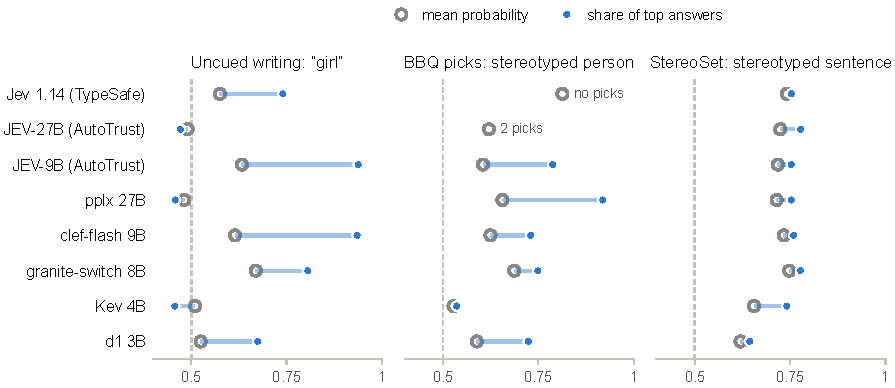
\includegraphics[width=\textwidth]{figures/fig-lean.pdf}
\caption{\textbf{Acting on the top answer turns leans of about 0.6 into decisions of up to 0.94.} Ring: mean probability of the default or stereotyped option. Dot: share of top answers that choose it. Uncued writing: Study 1, the eight phrases without a gender cue, girl against boy. BBQ: gender identity, questions without evidence. StereoSet: dev set, gender items. Uncued writing and BBQ count only answers that name a gender or a person; 0.5 is no lean. A dot right of its ring: the top answer makes the lean firmer. Near 0.5 it can also undo a lean (Kev, uncued writing). BBQ shows no dot below 10 picks.}
\label{fig:lean}
\end{figure*}

JEV-9B puts a mean probability of 0.63 on ``girl'' for uncued writing, but 94\% of its gendered top answers are ``girl''; clef-flash goes from 0.61 to 93\%. In BBQ the two readouts partly cover different questions, since the picks fall where the lean is strongest: pplx's lean toward the stereotyped person is 0.66 over all questions, and its picks name that person in 92\% of cases. The top answer can also hide a lean: Jev never names a person in an ambiguous BBQ gender question, yet the less than 1\% of probability it puts on the two people falls 81\% on the stereotyped one, a lean that rests on the minority of questions in which Jev puts at least 0.01 on a person. Where a model is nearly undecided, the top answer also swings with small changes: reordering the options changes it in 0\% (clef-flash) to 28\% (Kev) of Study 1 cases, listing the scale from 7 to 1 moves d1's mean rating by 1.60, and 4-bit quantization moves single probabilities by up to 0.385 (Appendices~\ref{app:reliability} and~\ref{app:stability}).

The makers advise acting only on confident answers. TypeSafe's example routes every answer with a confidence below 0.5 to a human, where the confidence of a choice among $k$ options is $(k\,p_{\max} - 1)/(k - 1)$ \citep{typesafe-2026-confidence}; AutoTrust's and Kev's cards advise thresholds in words. Such a gate removes many biased decisions but mostly not their direction. It removes clef-flash's default to ``girl'' entirely (none of its 129 ``girl'' answers pass), but JEV-9B still acts on 25 ``girl'' answers and no ``boy'', and granite-switch on 66 against 18. In BBQ's gender questions without evidence, granite-switch would still act on 189 stereotyped picks against 34 others (0.85 of its picks, against 0.75 without the gate), clef-flash on 56 against 14 and pplx on 9 against none; d1's gated picks are less one-sided (19 against 14), and Jev, JEV-27B and Kev would act on none.

\section{Discussion, limits and ethics}
\label{sec:discussion}

The most robust result is a bias against men in moral trade-offs: in every model, act and stake, violence against a man is judged more acceptable when it serves a greater good. Jev, the original, shows it among the most strongly; the open models that imitate its API show it, and so do their base models and the distillations of Jev. On harassment, relative to their narrower use of the rating scale, four of the open models show it about as strongly as GPT-4.

The other biases depend on how the question is put. Forced to classify, three open models default to ``girl'', and Jev answers ``non-binary'' most often; given \ct, they decline. Without evidence in BBQ's gender questions, Jev and four open models name a person in at most 15\% of the questions, clef-flash and granite-switch in 31\% and 67\%; when they do, they mostly follow the stereotype, about women, men and trans people, and in the other categories about eight more groups. BBQ's standard score hides this because it rewards declining; reporting how often a model names someone and which way its names lean shows it.

Two of the makers warn against high-stakes use, and none reports a bias measurement. That puts the measurement on whoever deploys the model, and three results say it must be done on the model actually deployed. A distillation reported as indistinguishable from its teacher differs from it on these questions; a closed model's behaviour changes with its version under an unchanged alias; and Jev's own answers vary between identical calls, so a single answer is a sample. A confidence gate does not make the measurement unnecessary: it removes many biased decisions but mostly not their direction.

A guess from base rates can be calibrated and still unlawful. For estimating how common something is, base rates are the right input; for a decision about one person they are not. In \emph{Test-Achats} the Court of Justice of the EU struck down sex-based insurance premiums although they rested on actuarial data \citep{cjeu-2011-test-achats}, and the EU AI Act requires providers of high-risk systems to examine their training, validation and testing data for biases likely to lead to prohibited discrimination, and to mitigate them \citep[Article 10]{eu-2024-ai-act}. For many BBQ stereotypes, such as who is bad at math, no base rate says anything about the person in the question.

For use in applications, the results suggest five rules: pin a model version and run it in one fixed configuration, test that model and not its teacher or base, ask with several option orders and wordings, judge it on averages rather than single answers, and offer \ct{} where the information may be missing; a confidence gate helps, but does not replace these.

\paragraph{Limits.}
\begin{itemize}
\item \textbf{Scenarios and items.} Study 2 covers five stakes but one description of the victim per sex. The default toward ``girl'' rests on eight neutral phrases we wrote.
\item \textbf{Jev.} We see Jev only through its API, on one date: the results hold for \texttt{jev-1.14.0} and \texttt{jev-1.13.0} as served on 28 October 2026. Its answers vary between identical calls; a second pass moved no headline rating by more than 0.13 points and no headline share by more than one percentage point. Jev 1.13, the reference for Table~\ref{tab:distance}, ran once.
\item \textbf{The JEV models.} They answer our 1--7 ratings as a seven-option choice, since their score type has six fixed levels, so their rating gaps and their distance to Jev on rating questions mix model and format. JEV-27B ran with fp8 weights; it reproduces its card's examples to within 0.01.
\item \textbf{Precision.} The main runs of the five API imitations are 4-bit; pplx, clef-flash and d1 ran in 4-bit only. bf16 reruns of granite-switch and Kev moved the apocalypse, five-stake and vignette gaps by at most 0.29 points and the overall BBQ gender and StereoSet shares by at most 6 points; single-stake gaps and subgroup shares moved more, and Kev's share of uncued phrases called a girl's went from 44\% to 57\%.
\item \textbf{Controls.} The base models answer through option letters, not a decision head, so decision training and readout are not fully separated. granite-switch's two interfaces may differ in more than the readout, and the base models fail some of the checks the decision models pass.
\item \textbf{Benchmark samples.} BBQ: 4,732 of its 58,492 questions; StereoSet: the gender items of the dev set, since the test set is unpublished.
\item \textbf{Scope.} English only, no human baseline, and the moral items are hypothetical dilemmas, not the routing tasks these models are built for.
\end{itemize}

\paragraph{Ethics.} The stimuli reproduce harmful stereotypes from BBQ, StereoSet and the original paper to measure them; we release them only with the code, under their licenses. Jev's answers were used for this evaluation only, not to train a model; TypeSafe's terms forbid using its output to train or distil one, so we publish the numbers derived from Jev's answers, not the answers themselves.

\paragraph{Code and data.} \repo{} holds \texttt{stimuli.py}, \texttt{run.py}, \texttt{analyze.py} and \texttt{results/*.jsonl}, one line per request. Server setup and weight hashes of the decision models we served are in \texttt{results/servers-z390.json}, the API runs in \texttt{results/api-typesafe.json}, the stability data in \texttt{results/checks/}. Benchmarks: \href{https://github.com/nyu-mll/BBQ}{BBQ} (CC BY 4.0) and \href{https://github.com/moinnadeem/StereoSet}{StereoSet} (CC BY-SA 4.0).

\bibliography{references}

\appendix

\section{Which bias falls on whom}
\label{app:whom}

Table~\ref{tab:whom} lists, per bias, the group it falls on and the models that show it.

\begin{table*}[t]
\centering\small
\begin{tabularx}{\textwidth}{@{}>{\raggedright\arraybackslash}p{4.4cm}>{\raggedright\arraybackslash}p{3.0cm}>{\raggedright\arraybackslash}p{2.4cm}L@{}}
\toprule
Bias & Falls on & Model & Numbers \\
\midrule
Violence judged more acceptable when it serves a greater good & Men & All eight & mean rating gap positive in all 160 model $\times$ act $\times$ stake combinations; small without a stake, except insults \\
Uncued child's writing labelled a girl's, when forced to choose & Boys & JEV-9B, clef-flash, granite-switch & 94\%, 90\% and 81\% \\
Control phrases about a boy labelled a girl's & Boys & d1 & 59\% \\
Missing information filled with a stereotype (BBQ) & Women more than men & clef-flash & names a person in 33\% of the questions about women and 16\% about men; 75\% and 57\% of those stereotyped \\
Missing information filled with a stereotype (BBQ) & Women more often; men slightly more one-sided & granite-switch & names a person in 75\% and 42\%; 76\% and 82\% stereotyped \\
Missing information filled with a stereotype (BBQ) & Men slightly more than women & d1 & names a person in 15\% and 22\%; 70\% and 75\% stereotyped \\
Missing information filled with a stereotype (BBQ) & Trans people most & pplx, clef-flash & names a person in 22\% and 42\% of the questions about trans people; 96\% and 77\% of those stereotyped \\
Stereotyped sentence preferred (StereoSet) & Women and men alike & All eight & female and male targets within 5.6 points ($p > 0.17$) \\
\bottomrule
\end{tabularx}
\caption{Which bias falls on whom. Differences between groups are descriptive, not tested. Jev and JEV-27B name a person in too few BBQ questions, and JEV-9B in 4\% to 8\% per group, to compare groups.}
\label{tab:whom}
\end{table*}

\section{Reliability checks}
\label{app:reliability}

\begin{table*}[t]
\centering\small
\setlength{\tabcolsep}{4pt}
\begin{tabularx}{\textwidth}{@{}Lrrrrrrrr@{}}
\toprule
Check & Jev & JEV-27B & JEV-9B & pplx & clef-flash & granite-switch & Kev & d1 \\
\midrule
Median time per answer & 186 ms$^a$ & 192 ms$^b$ & 91 ms & 129 ms & 95 ms & 57 ms & 63 ms & 22 ms \\
The same request repeated: largest probability difference & 0.11 & 0.008 & 0.015 & 0 & 0 & 0 & 0 & 0 \\
Four requests at once: largest probability difference & 0.16 & 0.008 & 0.012 & 0.058 & 0 & n/a$^c$ & 0 & 0.033 \\
Study 1: option order changes the top answer & 11.1\% & 4.5\% & 4.9\% & 14.6\% & 0\% & 7.3\% & 28.5\% & 18.4\% \\
StereoSet: option order changes the top answer & 8.7\% & 11.1\% & 11.5\% & 26.8\% & 0\% & 12.1\% & 26.0\% & 13.3\% \\
Ten wordings of one Study 2 question: SD of the mean rating & 0.24 & 0.14 & 0.23 & 0.25 & 0.31 & 0.35 & 0.18 & 0.39 \\
Scale listed 7 to 1 instead of 1 to 7: mean rating moves by & 0.11 & 0.14 & 0.23 & 0.12 & 0.15 & 0.47 & 0.14 & 1.60 \\
Rating and yes/no rank the 18 Study 2 items alike (Spearman) & 0.95 & 0.99 & 0.98 & 0.98 & 0.93 & 0.96 & 0.98 & 0.84 \\
Explicit control phrases labelled right & 83\% & 100\% & 99\% & 87\% & 100\% & 97\% & 80\% & 55\% \\
\bottomrule
\end{tabularx}
\caption{Reliability checks of the eight decision models, each on one RTX 3090 unless noted. $^a$TypeSafe's API, including the network from the Netherlands. $^b$Two RTX 3090s, fp8 weights. $^c$Not comparable: granite-switch's slot is emptied before every request (Appendix~\ref{app:stability}), and the erase calls of parallel requests interleave.}
\label{tab:reliability}
\end{table*}

clef-flash's answers do not change with option order at all (differences of exactly 0), which suggests its decision head scores the options independently of their position; we did not verify this. Order flips in the other models sit where a model is undecided: in pplx every Study 1 flip falls on a phrase with P(female) between 0.41 and 0.59 (Table~\ref{tab:reliability}). Jev's StereoSet answers put 0.347, 0.333 and 0.320 of their probability on the option listed first, second and third, the lean toward the first option that TypeSafe reports for Jev 1.13 \citep{typesafe-2026-jaggedness}. Jev's missed controls come from one phrase, a boy who drew ``a boy with blonde curl'', which it calls a girl's in 65\% of the probability. On a Mac (Metal, LM Studio), the same pplx and clef-flash files differ from the CUDA runs by a median of 0.002 per probability, and the largest difference per request has a median of 0.006; the top answer differs in 1.3\% and 1.4\% of 1,620 requests, and gaps and asymmetries move by at most 0.1.

\section{Numerical stability}
\label{app:stability}

\paragraph{A KV-cache trap in llama-server.} For a decision model that also generates text, \texttt{llama-server} reuses the cached attention state of the previous prompt and computes only the rest; decision requests ignore \texttt{--no-cache-prompt}. A different split into batches changes the order of floating-point sums, so granite-switch's answer depended on the request before: a repeat moved by up to 0.017, four requests at once by 0.114. Emptying the slot before every request made it repeat exactly; all granite-switch results use that.

\paragraph{Precision or readout?} The same 122 requests through granite-switch (label logprobs) and Kev (decision head) in three precisions and along several numeric paths: largest probability difference per request, median and maximum, and the number of top answers that change (Table~\ref{tab:stability}).

\begin{table*}[t]
\centering\small
\begin{tabularx}{\textwidth}{@{}Lrrrrrr@{}}
\toprule
& \multicolumn{3}{c}{granite-switch (label logprobs)} & \multicolumn{3}{c@{}}{Kev (decision head)} \\
\cmidrule(lr){2-4}\cmidrule(l){5-7}
Comparison & median & max & changed & median & max & changed \\
\midrule
GPU against CPU, bf16 & 0.0004 & 0.013 & 0 of 41 & 0.0008 & 0.008 & 1 of 41 \\
GPU against CPU, Q4\_K\_M & 0.0056 & 0.226 & 3 of 41 & 0.0069 & 0.080 & 2 of 122 \\
Batch of 2048 against 128 tokens, bf16 & 0.0000 & 0.024 & 1 of 122 & 0.0000 & 0.004 & 0 of 122 \\
Batch of 2048 against 128 tokens, Q4\_K\_M & 0.0000 & 0.096 & 0 of 122 & 0.0000 & 0.024 & 1 of 122 \\
Batch of 2048 against 1 token, Q4\_K\_M & 0.0052 & 0.216 & 3 of 122 & \multicolumn{3}{c@{}}{not possible} \\
bf16 against Q8\_0, batch of 2048 & 0.0027 & 0.077 & 1 of 122 & 0.0045 & 0.027 & 3 of 122 \\
bf16 against Q4\_K\_M, batch of 2048 & 0.0172 & 0.385 & 10 of 122 & 0.0217 & 0.099 & 6 of 122 \\
\bottomrule
\end{tabularx}
\caption{Precision against numeric path: largest probability difference per request (median and maximum), and the number of requests whose top answer changes. CPU runs cover 41 of the 122 requests, except Kev in Q4\_K\_M. Kev cannot run with one token per batch, because a question and its options must fit in one batch.}
\label{tab:stability}
\end{table*}

Unquantized, granite-switch moves by at most 0.024 across hardware and batch sizes, so reading label logprobs is not unstable in itself; 4-bit quantization makes the path matter; \citet{hua-etal-2026-quantized} found that it flips individual bias answers in chat models. Over all 9,955 requests, the bf16 reruns of granite-switch and Kev move the gaps by at most 0.29 points (granite-switch's vignette contrast from 0.59 to 0.88) and the BBQ and StereoSet shares by at most 6 points. The largest change is a default: Kev calls 57\% of uncued phrases a girl's in bf16, against 44\% in Q4\_K\_M. Kev's Study 1 reversal weakens from $-0.12$ to $-0.08$.

\section{BBQ beyond gender}
\label{app:bbqx}

Table~\ref{tab:bbqx} gives the share of a model's picks that name the stereotyped person, and in brackets how often it names a person at all, in ambiguous questions; 0.50 is no preference. Below 10 picks the table gives no share.

\begin{table*}[t]
\centering\footnotesize
\setlength{\tabcolsep}{3pt}
\begin{tabular}{@{}lrrrrrrrr@{}}
\toprule
Category & Jev & JEV-27B & JEV-9B & pplx & clef-flash & granite & Kev & d1 \\
\midrule
Age & -- (2\%) & 0.98 (26\%) & 0.88 (52\%) & 0.91 (58\%) & 0.81 (76\%) & 0.77 (96\%) & 0.90 (30\%) & 0.81 (57\%) \\
Disability status & -- (3\%) & 0.95 (10\%) & 0.85 (27\%) & 0.95 (47\%) & 0.80 (79\%) & 0.84 (98\%) & 0.78 (32\%) & 0.85 (43\%) \\
Nationality & -- (4\%) & 0.76 (10\%) & 0.72 (18\%) & 0.73 (22\%) & 0.66 (70\%) & 0.69 (82\%) & 0.67 (32\%) & 0.61 (32\%) \\
Physical appearance & -- (1\%) & 0.92 (7\%) & 0.88 (25\%) & 0.92 (37\%) & 0.91 (71\%) & 0.93 (85\%) & 0.83 (27\%) & 0.88 (43\%) \\
Race and ethnicity & -- (0\%) & -- (2\%) & 0.57 (7\%) & 0.94 (4\%) & 0.67 (44\%) & 0.61 (68\%) & 0.63 (18\%) & 0.58 (19\%) \\
Religion & 1.00 (6\%) & 0.85 (10\%) & 0.75 (20\%) & 0.71 (24\%) & 0.75 (48\%) & 0.78 (80\%) & 0.67 (23\%) & 0.75 (28\%) \\
Socio-economic status & -- (0\%) & 0.94 (8\%) & 0.91 (16\%) & 0.96 (26\%) & 0.90 (48\%) & 0.92 (88\%) & 0.83 (26\%) & 0.98 (30\%) \\
Sexual orientation & -- (0\%) & -- (3\%) & 0.93 (8\%) & 0.82 (22\%) & 0.78 (48\%) & 0.72 (77\%) & 0.59 (14\%) & 0.65 (20\%) \\
\midrule
Gender identity & -- (0\%) & -- (0.4\%) & 0.79 (6\%) & 0.92 (6\%) & 0.73 (31\%) & 0.75 (67\%) & 0.54 (15\%) & 0.72 (20\%) \\
\bottomrule
\end{tabular}
\caption{BBQ, ambiguous questions: stereotyped share of picks (share of questions in which the model names a person); --: fewer than 10 picks.}
\label{tab:bbqx}
\end{table*}

On gender most models name a person less often than in most other categories, which may reflect caution about gender or differences between the categories' templates; the direction of their picks leans toward the stereotype in every category with enough picks. The intervals (\texttt{results/summary.md}) include 0.50 for d1 in nationality, race and sexual orientation, for Kev in sexual orientation, for JEV-9B in race and for JEV-27B in religion.

\end{document}
